\documentclass[text05.tex]{subfiles}
\begin{document}
\newpage
\section{\ruby{距離}{きょ|り}センサーを使ってみよう}
\ruby{距離}{きょ|り}センサーをHSPで使ってみましょう。\ruby{距離}{きょ|り}センサー(番号は書いてありません。\pageref{distance}ページを参考にしてください)をA0につなげましょう。HSPスクリプトエディタで、\textasciitilde /05/kyori.hspを開いて実行してください。

\begin{figure}[H]
 \begin{minipage}[t]{0.3\columnwidth}
 \centering
 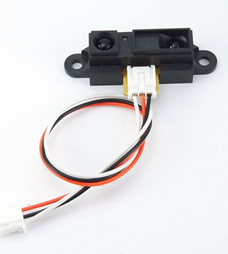
\includegraphics[width=\linewidth]{../../asset/image/text05-img031.png}
 \caption{\ruby{距離}{きょ|り}センサー}
 \end{minipage}
%\hspace{0.01\columnwidth} % ここで隙間作成
 \begin{minipage}[t]{0.5\columnwidth}
 \centering
 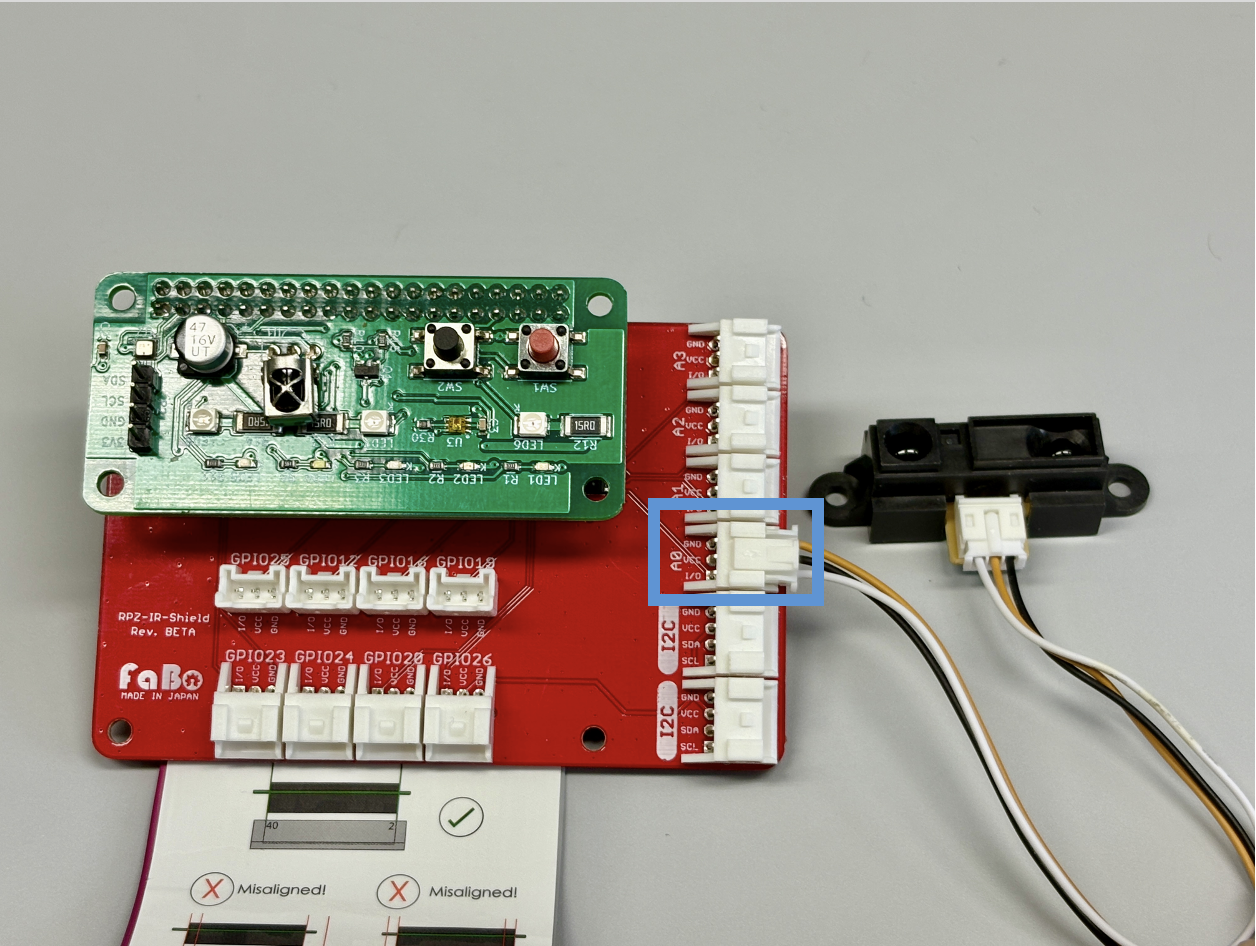
\includegraphics[width=\linewidth]{../../asset/image/text05-img054.png}
 \caption{アナログ入力A0}
 \end{minipage}
\end{figure}
\begin{lstlisting}[caption=kyori.hsp,label=kyori.hsp]
#include "hsp3dish.as"
#include "rpz-gpio.as"

spiopen 0	<#blue#;SPIチャンネルを開く#>

*main

	data = adcget(0,0)	<#blue#;SPIを使ってデータを受け取る#>
	kyori = 3952640 / (875*data + 22272)	<#blue#;dataを距離に変換する#>
	res = "距離 : "+kyori
	
	redraw 0
	font "",20
	pos 30,30
	mes res
	redraw 1

	wait 10
	goto *main

spiclose 0	<#blue#;SPIチャンネルを閉じる#>
\end{lstlisting}

\ruby{距離}{きょ|り}センサーのデータは\code{\adcget}を使って受け取ることができます。\ruby{値}{あたい}は0～1023になります。これでは\ruby{距離}{きょ|り}がわからないので、受け取った\ruby{値}{あたい}をcm(センチメートル)に\ruby{変換}{へん|かん}する必要があります。\ruby{変換}{へん|かん}するための式は\pageref{distance}ページに書いてあります。今回は入力は\code{data}という変数にしているので、式のxをdataにします。\code{kyori = 3952640 / (875*data + 22272)}で入力を\ruby{距離}{きょ|り}に\ruby{変換}{へん|かん}し、\code{kyori}変数に代入しています。単位はcmです。\\

\begin{tcolorbox}[title=\useOmetoi]
\begin{enumerate}
\addex{\ruby{距離}{きょ|り}センサーをA0につなげてkyori.hspを実行してみましょう。\ruby{測定}{そく|てい}できる\ruby{距離}{きょ|り}はだいたい10～80cmです。}
\end{enumerate}
\end{tcolorbox}
\end{document}
